%!TEX root = paper.tex
\section{Implementation Details}
\label{sec:implementation}
This section presents our preliminary implementation of InferSpark, which
as a first step, supports a class of Bayesian networks known as the 
exponential-conjugate family. These include the popular LDA model and its
variants. The primary inference algorithm for the exponential-conjugate family
is VMP and thus it's the target of our implementation at present.
In the future, the InferSpark language will be extended to support more Bayesian
networks and the appropriate inference algorithms will be included in our system
as well.

The main jobs of InferSpark are Bayesian network construction and 
code generation (\figref{fig:workflow}). 
We use the code generation approach because it enables a more flexible API
than a library. For a library, there are fixed number of API for user to
provide data, while InferSpark can dynamically generate custom-made API 
according to the structure of the Bayesian network. 
Another reason for using code generation is
that compiled programs are always more efficient than interpreted programs.
Afterwards, the generated program would be executed on Spark.
We next describe the implementation of
these modules and our runtime data partition strategies.

\subsection{Bayesian Network Construction}\label{sec:bnc}

In this offline compilation stage, the model definition is first transformed
into a Bayesian network.  We use the macro annotation, a compile-time meta
programming facility of Scala.  It is currently supported via the
macroparadise plugin. After the parser phase, the class annotated with ``{\sf
@Model}'' annotation is passed from the compiler to the transform method of
InferSpark. InferSpark treats the class passed to it as model definition and
transforms it into a Bayesian network.

\begin{figure}[!h]
\centering
\small
	\begin{tabular}{lrl}
		ModelDef		& ::= & `@Model' `class' id \\
					&     &`(' ClassParamsOpt `)' `\{' Stmts `\}' \\
		ClassParamsOpt	& ::= & `' /* Empty */ \\
						&	| &	ClassParams \\
		ClassParams		& ::= & ClassParam  [`,' ClassParams] \\
		ClassParam		& ::= & id `:' Type \\
		Type			& ::= & `Long' | `Double' \\
		Stmts			& ::= & Stmt [[semi] Stmts]\\
		Stmt			& ::= & `val' id = Expr \\
		Expr			& ::= & `\{' [Stmts [semi]] Expr `\}' \\
						&	| & DExpr	\\
						&   | & RVExpr \\
						&	| & PlateExpr \\
						&	| & Expr `.' `map' `(' id => Expr `)'\\
		DExpr			& ::= & Literal	\\
						&   | & id \\
						&   | & DExpr (`+' | `-' | `*' | `/') DExpr \\
						&   | & (`+' | `-') DExpr	\\
		RVExpr			& ::= & `Dirichlet' `(' DExpr `,' DExpr `)' \\
						&   | & `Beta' `(' DExpr `)' \\
						&   | & `Categorical' `(' Expr `)' \\
						&   | & RVExpr RVArgList	\\
						&   | & id	\\
		RVArgList		& ::= & `(' RVExpr `)' [ RVArgList ] \\
		PlateExpr		& ::= & DExpr `until' DExpr	\\ 
						&   | & DExpr `to' DExpr	\\
						&	| & `?' \\
						&	| & id
	\end{tabular}
\caption{InferSpark model definition syntax}
\label{fig:inferspark_syntax}
\end{figure}

\figref{fig:inferspark_syntax} shows the syntax of InferSpark model
definition. The expressions in a model definition is divided into 3
categories: deterministic expressions (DExpr), random variable expressions
(RVExpr) and plate expressions. The deterministic expressions include
literals, class parameters and their arithmetic operations. The random
variable expressions define random variables or plates of random variables.
The plate expressions define plate of known size or unknown size. The random
variables defined by an expression can be binded to an identifier by the value
definition. It is also possible for a random variable to be binded to multiple
or no identifiers. To uniquely represent the random variables, we assign
internal names to them instead of using the identifiers.

\begin{figure}[ht]
\centering
	\includegraphics[width=0.6\columnwidth]{figs/two_coins_internal_bn1.eps}
	\caption{Internal representation of Bayesian network}
	\label{fig:two_coins_internal_bn1}
\end{figure}

Internally, InferSpark represents a Bayesian network in a tree form, where the
leaf nodes are random variables and the non-leaf nodes are plates. The edges
in the tree represent the nesting relation between plates or between a plate
and random variables. The conditional dependencies in the Bayesian network are
stored in each node.  The root of the tree is a predefined plate TOPLEVEL with
size 1.  \figref{fig:two_coins_internal_bn1} is the internal representation of
the two-coin model in \figref{fig:two_coins_bn1}, where
$r_1$, $r_2$, $r_3$, $r_4$, correspond to $\pi$, $\phi$, $z$, $x$, respectively. 
Plate 1 and Plate 2 corresponds to the plates defined on lines 3--5 in
\figref{fig:two_coins_modeldef}. 

If a plate is nested within another plate,
the inner plate is repeated multiple times, in which case,
the size attribute of the plate node will be computed by summing the size of each
repeated inner plate. We call the size attribute in the tree {\em flattened size}
of a plate. For example, in \figref{fig:two_coins_nestedplates}, the flattened
size of the innermost plate around $x$ is $\sum_i N_i$.


InferSpark recursively descends on the abstract syntax tree (AST) of the model definition to construct
the Bayesian network.   In the
model definition, InferSpark follows the normal lexical scoping rules.
InferSpark evaluates the expressions to one of the following three results
\begin{itemize}
	\item a node in the tree
	\item a pair $(r, \textrm{plate})$ where $r$ is a random variable node
		and plate is a plate node among its ancestors, which represents all
		the random variables in the plate
	\item a deterministic expression that will be evaluated at run time
\end{itemize}

At this point, apart from constructing the Bayesian network representation, 
InferSpark also generates the code for metadata collection, a module used in 
stage 2. For each random variable name bindings, a singleton interface object 
is also created in the resulting class. 
The interface object provides ``{\sf observe}'' and ``{\sf getResult}'' API for later use.

\subsection{Algorithm Matching \& Code Generation}

The algorithm matching module iterates through all the built-in and
developer-supplied algorithms and checks if the algorithm is applicable.  For
the VMP algorithm, it needs to check whether the model is in
exponential-conjugate family. 

Code Generation is divided into 4 steps: metadata
collection, message annotation, MPG construction code generation and inference
execution code generation.

Metadata collection aims to collect the values of the model parameters,
check whether random variables are observed or not, the flattened sizes of the plates.
These metadata can help to 
assign vertex ID to the vertices in the message passing graph.  
After the flattened sizes of plates are calculated, we can assign vertex IDs to the
vertices that will be constructed in the message passing graph. Each random
variable will be instantiated into a number of vertices in the MPG where the
number equals to the flattened size of its innermost plate. The vertices
of the same random variable are assigned consecutive IDs. For example, $x$ may
be assigned ID from $0$ to $N-1$. The intervals of IDs of random variables in
the same plate are also consecutive. A possible ID assignment to $z$ is $N$ to
$2N - 1$. Using this ID assignment, we can easily i) determine which random
variable the vertex is from only by determining which interval the ID lies
in; ii) find the ID of the corresponding random variable in the same plate by
subtracting or adding multiples of the flattened plate size (e.g. if $x_i$' ID is
$a$ then $z_i$'s ID is $a + N$).

Message annotation aims to annotate the Bayesian Network Template from the previous stage (Section \ref{sec:bnc})
with messages
to be used in VMP algorithm.  The annotated messages are stored in the form of
AST and will be incorporated into the the generated code, output of this stage. 
The rules of the messages to annotate are predefined according to the
derivation of the VMP algorithm.
After the messages are generated, we
generate for each type of random variable a class with the routines for
calculating the messages and updating the vertex. 

The generated code for constructing  the message passing graph requires  building a VertexRDD
and an EdgeEDD. The VertexRDD is an RDD of vertex ID and vertex attribute pairs.
Vertices of different random variables
are from different RDDs (e.g., {\sf v1}, {\sf v2}, and {\sf v3} in \figref{fig:two_coins_mpg_constr_code})
and have different initialization methods.
For unobserved random variables, the source can be any RDD that has the same
number of elements as the vertices instantiated from the random variable. For
observed random variables, the source must be the data provided by the user. If
the observed random variable is in a plate, the vertex id can be
calculated by first combining the indices to the data RDD then adding an offset.

One optimization of constructing the EdgeRDD is to \emph{reverse the edges}.
If the code generation process generates an EdgeRDD in straightforward manner,
the {\sf aggregateMessages} function has to scan all the edges to find edges
whose destinations are of $v$ type because GraphX indexes the \emph{source}
but not the \emph{destination}.  Therefore, we generate code that reverses the
edge and specify the active edge direction as source only in the call to
{\sf aggregateMessages} so as to enjoy the indexing feature of GraphX.  When
constructing the graphs, we also take into account the graph partitioning
scheme because that has a strong influence on the performance.  We discuss
this issue in the next section.


The final part is to generate the inference execution code that implements the
iterative update of the VMP algorithm. 
We aim to generate code that updates each vertex in the
message passing graph at least once in each iteration. 
As it is safe to update vertices that do not
have mutual dependencies, i.e., those who do not send messages to one another,
we divide each iteration into substeps.
Each substep updates a portion of the
message passing graph that does not have mutual dependencies. 

A substep in each iteration consists of two GraphX operations:
{\sf aggregateMessages} and {\sf outerJoinVertices}. Suppose {\sf g} is the message passing
graph, the code of a substep is:

\begin{figure}[h]
\centering
\begin{lstlisting}
val prevg = g
val msg = g.aggregateMessages(sendMsg, mergeMsg, TripletFields)
g = g.outerJoinVertices(msg)(updateVertex).persist()
g.edges.count()
prevg.unpersist()
\end{lstlisting}
\caption{The code generated for a substep in the VMP algorithm}
\label{fig:code_substep}
\end{figure}

The RDD {\sf msg} does not need to be cached because it is only used once. But
the code generated has to cache the graph {\sf g} because the graph is used in
both {\sf aggregateMessages} and {\sf outerJoinVertices}. However, only
caching it is not enough, the code generation has to include code like line 4
above to activate the caching process.  Once {\sf g} is cached, code
generation evicts the previous (obsolete) graph {\sf prevg} from the cache.
To avoid the long lineage caused by iteratively updating message passing
graph, which will overflow the heap space of the drive, the code generation
process also adds a line of code to checkpoint the graph to HDFS every $k$
iterations for some user-specified $k$.

\subsection{Execution}

The code generated at run time are sent to the Scala compiler. The resulting
byte code is added to the class path of both the driver and the workers. Then
InferSpark initiates the inference iterations via reflection invocation.


\subsection{Discussion on Partitioning Strategies}

\begin{figure}[h]
	\centering
	\includegraphics[width=0.45\textwidth]{figs/mixture_mpg.eps}
	\caption{Message passing graph of a mixture model}
	\label{fig:mixture_mpg}
\end{figure}

GraphX adopts a vertex-cut partitioning approach.
The vertices are replicated in edge partitions instead of edges being replicated in vertex
partitions. 
The four built-in partition
strategies in GraphX are: 
EdgePartition1D (1D),
EdgePartition2D  (2D),
RandomVertexCut (RVC), and
CanonicalRandomVertexCut (CRVC).
In the following, we first show that these general 
partitioning strategies perform badly for the VMP algorithm on MPG.
Then, we introduce our own partitioning strategy.

\figref{fig:mixture_mpg} shows a more typical message passing graph of a
mixture model instead of the toy two-coin model that we have used so far. $N$
is the number of $x$ and $z$, $K$ is the number of $\phi$, $D$ is the number
of $\theta$. Typically, $N$ is very large because that is the data size (e.g.,
number of words in LDA), $K$ is a small constant (e.g., number of topics in
LDA), and $D$ could be a constant or as large as $N$ (e.g., number of
documents in LDA). Note that we reverse the edges in the MPG. Since there are
edges in both direction whenever two vertices are linked, we still refer to
the original edges in the following discussion.  Another implication is that
ONLY the \emph{destination} end of an edge (the source end in the actual
graph) is replicated in the edge partition where the edge resides since we
specify the active edge direction as destination only (source only in the
actual implementation). In the following discussion, let $M$ be the number of
edge partitions and we assume that the ratio $\eta = \frac{N}{M}$ has a limit
(e.g. the maximum number of $x$'s that fits within the maximum RDD block size).

EdgePartition1D is essentially a random partitioning strategy, except that it
co-locates all the edges with the same source vertex. Suppose all the edges from
$\phi_k$ are assigned to partition $k$. Since there's an edge from $\phi_k$ to
each one of the $N$ vertices $x$, partition $k$ will have the replications
of all $x_1, x_2, \ldots, x_N$. In the best case, 
edges from different $\phi_k$ are assigned to different
partitions. Then the largest edge partition still have at least $N$ vertices.
When $N$ is very large, the largest edge partition is also very large, which
will easily cause the size of an edge partition to exceed the RDD block size limit. 
Moreover, the best case turns out to be the worst case 
when it comes to the number of vertex replications
because it actually replicates the size $N$ data $K$ times, which is
extremely space inefficient. The over-replication also incurs large amount of
data shuffle when we perform outer joins because each updated vertex has to
be shipped to every edge partition, prolonging the running time. 

We give a more formal analysis of the number of vertices in the largest edge
partition and the expected number of replications of $x_i$ under
EdgePartition1D. As discussed above, there's at least one edge partition that
has replications of all the $x_i$'s. 
Observe that the graph has an upper bound of
$3N + K$ vertices, so the number of vertices in the largest edge partition is
$O(N)$. Let $N_{x_i}$ be the number of replications of $x_i$, then the expected
number of replication of $x_i$ is 
\begin{align*}
	E[N_{x_i}] &= M(1 - (1 - \frac{1}{M})^{K+1}) \\
		&= \left\{
			\begin{array}{ll}
				(K + 1) + o(1) & K = O(1) \\
				M + o(1) & K = O(M) 
			\end{array}
		\right.%}
\end{align*}

\begin{figure}[h]
	\centering
	\includegraphics[scale=0.25]{figs/2dhash.eps}
	\caption{EdgePartition2D. Each grid is a partition. 
	The possible partitions where $x_i$ is
	replicated is shaded}
	\label{fig:2dhash}
\end{figure}

EdgePartition2D evenly divides the adjacency matrix of the graph into $\sqrt{M}
\times \sqrt{M}$ partitions. The vertices are uniformly distributed along the
edges of the adjacency matrix by hashing into $\sqrt{M}$ buckets. The upper
bound of the number of replications of a vertex $x_i$ is $\sqrt{M}$ because all
the edges that point to it are distributed to at most $\sqrt{M}$ partitions
in shown as \figref{fig:2dhash}.  Meanwhile, there are $K+1$
edges pointing to $x_i$, so the number of replications of $x_i$ cannot exceed
$K+1$ as well. Therefore, the upper bound of replications of $x_i$ is actually
$\min(K+1, \sqrt{M})$. On the other hand, suppose each of the $\phi_k$ is
hashed to different bucket and $N$ $x$'s are evenly distributed into the
$\sqrt{M}$ buckets, then the number of largest partition is at least
$\frac{N}{\sqrt{M}}$, which is still huge when the average number of words per
partition is fixed. Following is the formal analysis of the EdgePartition2D.

Let $B$ be an arbitrary
partition in the dark column on \figref{fig:2dhash}.
Let $Y_{x_i, B}$ be the indicator variable for the event that $x_i$ is
replicated in $B$.
Then the expectation of $Y_{x_i, B}$ is
\begin{align*}
	E[Y_{x_i, B}] &= 1 - (1 - \frac{1}{\sqrt{M}})^{K+1} \\
\end{align*}

The number of vertices $N_B$ in the largest partition $B$ is at least the expectation
of the number of vertices in a partition, which is also at least the
expectation of the number of $x_i$ in it:
\begin{align*}
	E[N_{B}] &= \sum_{v} E[Y_{v, B}] \\
		&\ge \frac{N}{\sqrt{M}} E[Y_{x_i, B}]	\\
		& = \left\{
				\begin{array}{ll}
					(K + 1)\eta	+ o(1) & K = O(1) \\
					\sqrt{M}\eta + o(1) & K = O(M) 
				\end{array}
			\right.%}
\end{align*}

The expected number of replications of $x_i$ is
\begin{align*}
	E[N_{x_i}] &= \sqrt{M}E[Y_{x_i, B}] \\
		&= \left\{
			\begin{array}{ll}
				(K + 1) + o(1) & K = O(1) \\
				\sqrt{M} + o(1) & K = O(M) 
			\end{array}
		\right.%}
\end{align*}


%
RandomVertexCut (RVC) uniformly assigns each edge to one of the $M$
partitions. The expected number of replications of $x_i$ tends to be $O(K)$
when $K$ is a constant and tends to be $O(N)$ when $K$ is proportional to the
number of partitions. The number of vertices in the largest partition is also
excessively large. It is $O(K\frac{N}{M})$ when K is a constant and $O(N)$
when $K$ is proportional to the number of partitions.  CanonicalRandomVertexCut
assigns two edges between the same pair of vertices with opposite directions
to the same partition. For VMP, it is the same as RandomVertexCut since only
the destination end of an edge is replicated. For example, if $x_i$ has $K +1$
incoming edges, then the probability that $x_i$ will be replicated in a
particular partition is independent from whether edges in opposite
direction are in the same partition or randomly distributed. Therefore 
CRVC will have the same result as RVC.  
\tabref{tab:max_v_per_edge_part_O1} and
\tabref{tab:max_v_per_edge_part_OM} summarize the comparison of different
partition strategies.

InferSpark's partitioning strategy is actually tailor-made for VMP's message passing graph.
The intuition is that the MPG has a special structure.
For example, in \figref{fig:mixture_mpg},
we see that the MPG essentially has $D$ ``independent'' trees rooted at $\theta_i$,
where the leaf nodes  are $x$'s and they form a complete bipartite graph with all $\phi$'s.
In this case, one good partitioning strategy is to form $D$ partitions, 
with each tree going to one partition and the $\phi$'s getting replicated $D$ times.
We can see that such a partition strategy incurs no replication on $\theta$, $z$, and $x$,
and incurs $D$ replications on $\theta$.

Generally, our partitioning works as follows: Given an edge, we first determine
which two random variables (e.g. $x$ and $z$) are connected by the edge. It is
quite straightforward because we assign ID to the set of vertices of the same
random variable to a consecutive interval. We only need to look up which
interval it is in and what the interval corresponds to. Then we compare the
total number of vertices corresponding to the two random variables and choose
the larger one. Let the Vertex ID range of the larger one to be $L$ to $H$. We
divide the range from $L$ to $H$ into $M$ sub ranges. The first sub-range is $L$
to $L + \frac{H-L+1}{M}$; the second is $L + \frac{H-L+1}{M} + 1$ to $L +
2\frac{H-L+1}{M}$ and so on. If the vertex ID of the edge's chosen vertex falls
into the $m^{th}$ subrange, the edge is assigned to partition $m$.

In the mixture case, at least one end of every edge is $z$ or $x$. Since
the number of $z$'s and $x$'s are the same, 
each set of edges that link to the $z_i$ or $x_i$ with 
the same $i$ are co-located. This guarantees that $z_i$
and $x_i$ only appears in one partition. All the $\phi_k$'s are replicated in each
of the $M$ partitions as before. The only problem is that many $\theta_j$ with
small $N_j$ could be replicated to the same location. In the worst case, the
number of $\theta$ in one single partition is exactly $\eta$. However, it is
not an issue in that case because the number of vertices in the largest
partition is still a constant $3\eta + K$. It is also independent from whether $K
= O(1)$ or $K = O(M)$.


\begin{table}[h]
	\centering
	\caption{Analysis of different partition strategies when $K = O(1)$}
	\label{tab:max_v_per_edge_part_O1}
	\small
	\begin{tabular}{lll}
		\hline
		Partition Strategy & $E[N_{x_i}]$ & $E[N_B]$\\\hline\hline
		1D & $O(K)$ & $O(N)$ \\\hline
		2D & $O(K)$ & $O(K\frac{N}{M})$ \\\hline
		RVC & $O(K)$ & $O(K\frac{N}{M})$ \\\hline
		CRVC & $O(K)$ & $O(K\frac{N}{M})$ \\\hline
		{\bf InferSpark} & 1 & $3\frac{N}{M}+1$ \\\hline
	\end{tabular}
\end{table}

\begin{table}[h]
	\centering
	\caption{Analysis of different partition strategies when $K = O(M)$}
	\label{tab:max_v_per_edge_part_OM}
	\small
	\begin{tabular}{lll}
		\hline
		Partition Strategy & $E[N_{x_i}]$ & $E[N_B]$\\\hline\hline
		1D & $O(M)$ & $O(N)$ \\\hline
		2D & $O(\sqrt{M})$ & $O(\sqrt{M}\frac{N}{M})$ \\\hline
		RVC & $O(M)$ & $O(N)$ \\\hline
		CRVC & $O(M)$ & $O(N)$ \\\hline
		{\bf InferSpark} & 1 & $3\frac{N}{M}+1$ \\\hline
	\end{tabular}
\end{table}

